\documentclass{beamer}
\usepackage[english]{babel}
\usepackage[latin1]{inputenc}
\usepackage[T1]{fontenc}
\usepackage{movie15}
\usepackage{graphicx}
\usepackage{caption}
\usepackage{subfig}
\usepackage{xcolor}
\usepackage{amsmath}
\usepackage{tikz}
\usepackage[]{algorithm2e}
\usepackage{listings}
\usepackage{chngpage}

\setbeamertemplate{caption}[numbered]

\tikzstyle{mybox} = [draw=green, very thick, rectangle, rounded corners, inner ysep=5pt, inner xsep=5pt, fill=green!20]

\newenvironment{cambiamargini}[2]{% 
  \begin{list}{}{% 
    \setlength{\topsep}{0pt}% 
    \setlength{\leftmargin}{#1}% 
    \setlength{\rightmargin}{#2}% 
    \setlength{\listparindent}{\parindent}% 
    \setlength{\itemindent}{\parindent}% 
    \setlength{\parsep}{\parskip}% 
  }% 
  \item[]}{\end{list}}

\newenvironment<>{varblock}[2][.9\textwidth]{%
  \setlength{\textwidth}{#1}
  \begin{actionenv}#3%
    \def\insertblocktitle{#2}%
    \par%
    \usebeamertemplate{block begin}}
  {\par%
    \usebeamertemplate{block end}%
  \end{actionenv}}


\author[Massimiliano Lupo Pasini]{Massimiliano Lupo Pasini (Emory University)\\
\institute{Emory University}
\vspace{0.5cm}\tiny{In collaboration with: \\Michele Benzi (Emory 
University)\\Thomas 
Evans (Oak Ridge National Laboratory), \\Steven Hamilton(Oak Ridge National 
Laboratory), \\Stuart Slattery(Oak Ridge National Laboratory)} 
\\\vspace{0.5cm}Research supported by DOE (Office of Science)}
\vspace{0.1cm}
\institute{SIAM Conference on Computational Science and Engineering 2015}
%Oak Ridge National Laboratory
\title[MCSA]{ \small Iterative Performance of Monte Carlo Linear Solver Methods}
%\titlegraphic{
\includegraphics[scale=0.5]{imago/Emory-logo}}
\date[3.17.2015]{\small March 17, 2015}

\usetheme{Berlin}
\useinnertheme{rounded}
\setbeamercovered{dynamic}

\begin{document}

% % % % % % % % % % % % % % % % %
% % %		COPERTINA 		% % %
% % % % % % % % % % % % % % % % %

\begin{frame}
\maketitle
\end{frame}

% % % % % % % % % % % % % % % % %
% % %		CONTENUTI 		% % %
% % % % % % % % % % % % % % % % %


\begin{frame}
\small\frametitle{Outline}
\begin{itemize}[<+->]
\item Motivations
\vspace{0.3cm}
\item Standard Monte Carlo vs. Monte Carlo Synthetic Acceleration (MCSA)
\vspace{0.3cm}
\item Choice of the preconditioner
\vspace{0.3cm}
\item Convergence conditions
\vspace{0.3cm}
\item Numerical results
\end{itemize}
\end{frame}


\section{Motivations}

\begin{frame}
\frametitle{Motivations}
Goal:
\begin{itemize}
\item development of reliable algorithms to solve highly dimensional (towards 
exascale) sparse linear systems in parallel
\end{itemize}
\vspace{0.5cm}
Issues:
\begin{itemize}
\item occurrence of \textbf{faults} (abnormal operating conditions of the 
computing system which cause a wrong answer)
\begin{itemize}
\item hard faults
\item soft faults
\end{itemize}
\end{itemize}
\vspace{0.5cm}
[M. Hoemmen and M.A. Heroux, 2011; G. Bronevetsky and B.R. de Supinski, 2008; P. Prata and J.B. Silva, 1999 ]
\end{frame}

\begin{frame}
\frametitle{Motivations}

\begin{varblock}[11cm]{}
\textcolor{red}{\textbf{Resilience}: ability to compute a correct output in 
presence of faults}
\end{varblock}
\vspace{0.5cm}

Different approaches to tackle the problem:
\begin{itemize}
\item 
 adaptation of Krylov subspace methods (CG, GMRES, Bi-CGStab, ...) to fault 
tolerance by recover-restart strategies

\item abandonment of deterministic paradigm in favor of stochastic approaches
\end{itemize}
\vspace{0.5cm}
\small{[E. Agullo, L. Giraud, A. Guernouche, J. Roman and  M. Zounon, 2013]}
\end{frame}

\section{Standard MC vs. MCSA}
\begin{frame}
\frametitle{Monte Carlo Linear Solvers}
\framesubtitle{Mathematical setting}
Let us consider a sparse linear system 
\begin{equation}
A \mathbf{x}=\mathbf{b},
\label{linsys}
\end{equation}
where $A\in \mathbb{R}^{n\times n}$, $\mathbf{x}\in 
\mathbb{R}^n$, $\mathbf{b} \in 
\mathbb{R}^n$. 

With left preconditioning (\ref{linsys}) becomes 
\begin{equation}
\color{red}{P^{-1}}\color{black}{A\mathbf{x}}=\color{red}{P^{-1}}\color{black}
\mathbf {b}, \quad P\in\mathbb{R}^{n\times n}.
\label{prec_sys}
\end{equation}
(\ref{prec_sys}) can be reinterpreted as a fixed 
point scheme
\begin{equation}
 \mathbf{x}=\color{red}{H}\color{black}{\mathbf{x}+\mathbf{f}}
 \label{fixedpoint}, \quad H=I-P^{-1}A, \; \mathbf{f}=P^{-1}\mathbf{b}.
\end{equation}
Assuming $\rho(H)<1$, (\ref{fixedpoint}) generates a 
sequence of approximate solutions $\{\mathbf{x}_k\}_{k=0}^\infty$ which 
converges to the exact solution of (\ref{linsys}). 

\end{frame}

\begin{frame}
\frametitle{Monte Carlo Linear Solvers}
\framesubtitle{Mathematical setting}
 The solution to (\ref{fixedpoint}) can be written in terms of a power series 
in
$H$ (Neumann series):
\[
\mathbf{x}=\sum_{\ell=0}^\infty H^{\ell}\mathbf{f}.
\]

By restricting the attention to a single component of $\mathbf{x}$ we 
have
\begin{equation}
x_i=\sum_{\ell=0}^\infty \sum_{k_1=1}^n\sum_{k_2=1}^n\cdots \sum_{k_{\ell}=1}^n 
H_{k_0,k_1}H_{k_1,k_2}\ldots H_{k_{\ell-1}, k_{\ell}}f_{k_{\ell}}.
\label{Neumann}
\end{equation}

(\ref{Neumann}) can be reinterpreted as the \textcolor{red}{sampling of an 
estimator defined on a random walk}.
\end{frame}


\begin{frame}
\frametitle{Monte Carlo Linear Solvers}
\framesubtitle{Mathematical setting: Forward (Direct) Method}

\textcolor{red}{Goal}: evaluate a functional such as
\[
 J(\mathbf{x})=\left\langle \mathbf{h},\mathbf{x}\right\rangle =\sum_{i=1}^n 
h_i x_i, \quad 
\mathbf{h}\in\mathbb{R}^n.
\]
\textcolor{red}{Approach}: define random walks to evaluate $J$.

Consider a random walk whose 
state space $S$ is the set of indices of the forcing term 
$\mathbf{f}$:
\[
S=\{1,2,\ldots, n\} \subset \mathbb{N}.
\]
\small{[N. Metropolis and S. Ulam, 1949; G. E. Forsythe and A. Leibler, 1950; 
W. R. Wasow, 1952; J. H. Halton, 1962]}
\end{frame}

\begin{frame}
\frametitle{Monte Carlo Linear Solvers}
\framesubtitle{Mathematical setting: Forward (Direct) Method}

Initial probability: pick $k_0$ as initial step of the random walk:
\[
 \tilde{p}(k_0=i)=\tilde{p}_{k_0}=\frac{\lvert h_i \rvert}{\sum_{i=1}^n \lvert 
h_i \rvert}.
\]

Possible choices for the transition probability: $p(:,i):S\rightarrow 
[0,1]\quad \forall i \in S$
\begin{equation*}
\begin{align}
 & p(k_i=j | k_{i-1}=i)=P_{i,j}=\frac{\lvert 
H_{i,j}\rvert}{\sum_{i=1}^n\lvert H_{i,j}\rvert} 
\qquad\quad  \textcolor{blue}{weighted}
\end{align}
\end{equation*}



\begin{equation*}
\begin{align}
P_{i,j}=
\begin{cases}
0 \quad \quad \quad \qquad \qquad \qquad \text{if}\quad H_{i,j}=0 \\
\frac{1}{\#(\text{non-zeros in the row)}} \quad \text{if} \quad H_{i,j}\ne 0
\end{cases}\textcolor{blue}{uniform}
\end{align}
\end{equation*}
\end{frame}


\begin{frame}
\frametitle{Monte Carlo Linear Solvers}
\framesubtitle{Mathematical setting: Forward (Direct) Method}
A related sequence of weights is defined by
\[
 w_{i,j}=\frac{H_{i,j}}{P_{i,j}}
\]
in order to build an auxiliary sequence 
\[
 W_0=\frac{h_{k_0}}{\tilde{p}_{k_0}}, \quad W_{i}=W_{i-1}w_{k_{i-1},k_i}\quad 
k_{i-1},k_i \in S.
\]

This allows us to define a random variable $X(\cdot):\Pi\rightarrow 
\mathbb{R}$. 

$\Pi$= set of realizations of a random walk $\gamma$ defined on $S$:
\[
 X(\nu)=\sum_{\ell=0}^\infty W_{\ell} f_{k_{\ell}}, \quad \nu=\text{permutation 
of}\; 
\gamma
\]
\end{frame}


\begin{frame}
\frametitle{Monte Carlo Linear Solvers}
\framesubtitle{Mathematical setting: Forward (Direct) Method}
Define the expected value of $X(\cdot)$:
\[
E[X]=\sum_{\nu}P_{\nu}X(\nu)\quad (P_{\nu}= \text{probability of the 
permutation}\; \nu).
\]


It can be proved that
\[
 E[W_{\ell} f_{k_{\ell}}]=\left\langle \mathbf{h}, 
H^{\ell}\mathbf{f}\right\rangle
\]
and consequently
\[
 E\bigg[\sum_{{\ell}=0}^{\infty}W_{\ell} 
f_{k_{\ell}}\bigg]=\left\langle\mathbf{h}, 
\mathbf{x}\right\rangle.
\]

\end{frame}


\begin{frame}
\frametitle{Monte Carlo Linear Solvers}
\framesubtitle{Mathematical setting: Forward (Direct) Method}

\textcolor{blue}{If $\mathbf{h}$ is a vector of the standard basis}: 
$\mathbf{h}=\mathbf{e}_j$
\[
\tilde{p}(K_0=i)=\delta_{i,j},\quad i,j=1,\ldots,n
\]
and the expected value assumes the following form:
\begin{equation}
\tiny E\Big[\sum_{\ell=0}^\infty W_{\ell} 
f_{k_{\ell}}\Big]=x_i=\sum_{\ell=0}^\infty 
\sum_{k_1=1}^{n}\sum_{k_2=1}^n\cdots \sum_{k_{\ell}=1}^n 
P_{k_0,k_1}P_{k_1,k_2}\ldots P_{k_{{\ell}-1}, 
k_{\ell}}w_{k_0,k_1}w_{k_1,k_2}\ldots 
w_{k_{\ell-1}, k_{\ell}}f_{k_{\ell}}.
\label{dir_mean}
\end{equation}

\vspace{0.5cm}
\underline{\textbf{\color{red}Drawback}: the estimator is defined entry-wise}.
\end{frame}


\begin{frame}
\frametitle{Monte Carlo Linear Solvers}
\framesubtitle{Mathematical setting: Adjoint Method}
Consider the adjoint linear system
\begin{equation*}
 (P^{-1}A)^T\mathbf{y}=\mathbf{d}. 
 \label{lin_sys_adj}
\end{equation*}
With a fixed point approach, we get
\[
 \mathbf{y}=H^T\mathbf{y}+\mathbf{d}.
\]
By picking $\mathbf{d}=\mathbf{e}_j$  we have
\[ 
J^*(\mathbf{y}):=\left\langle\mathbf{y},\mathbf{f}
\right\rangle=\left\langle\mathbf { x } , \mathbf { e }
_j\right\rangle=x_j , \quad j=1,\ldots,n.
\]

\end{frame}


\begin{frame}
\frametitle{Monte Carlo Linear Solvers}
\framesubtitle{Mathematical setting: Adjoint Method}
The initial probability and transition matrix may be defined as
\[
\tilde{p}_{k0}=p(k_0=i)=\frac{\lvert f_i\rvert}{\sum_{i=1}^n \lvert f_i 
\rvert},\quad
P_{i,j}=\frac{\lvert 
\color{red}{H^T_{i,j}}\color{black}\rvert}{\sum_{k=1}^n\lvert 
\color{red}{H^T_{i,k}}\color{black}\rvert}=\frac{\lvert 
H_{j,i}\rvert}{\sum_{k=1}^n\lvert 
H_{k,i}\rvert}.
\]
Reintroduce weights as before:
\[
w_{i,j}=\frac{\color{red}{H_{j,i}}}{P_{i,j}}\Rightarrow 
W_{0}=sign(f_i)\lVert\mathbf{f}\rVert_1, \quad W_j=W_{j-1} w_{k_{i-1},k_i}, 
\quad k_{i-1},k_i \in S.
\]
Expected value of the estimator for the \underline{\color{red}{entire}} 
solution vector $\mathbf{x}$:
\begin{equation}
\tiny E\Big[\sum_{{\ell}=0}^\infty W_{\ell}
d_{k_{\ell}}\Big]=\sum_{{\ell}=0}^{\infty}\sum_{k_1}^n\sum_{k_2}^n\cdots\sum_{
k_{\ell} } ^n 
f_{k_0}P_{k_0,k_1}P_{k_1,k_2}\ldots P_{k_{\ell-1},K_{\ell}}w_{k_0,k_1}\ldots 
w_{k_{\ell-1},k_{\ell}}\delta_{k_{\ell},j}.
\label{adj_mean}
\end{equation}

\end{frame}

\begin{frame}
\frametitle{Monte Carlo Linear Solvers}
\framesubtitle{Statistical constraints for convergence}
Expected value and variance of the estimator must be finite to apply the 
Central Limit Theorem.
\vspace{0.5cm}

\begin{minipage}[t]{0.48\linewidth}
\hspace{5pt} \tiny Forward Method: $(H^*)_{i,j}=\frac{(H_{i,j})^2}{P_{i,j}}$
\begin{equation*}
 \tiny{E\bigg[\sum_{\ell=0}^\infty W_{\ell} f_{k_{\ell}}\bigg]<\infty 
\;\Leftrightarrow \; 
\rho(H)<1}
\end{equation*}
\begin{equation*}
 \tiny{Var\bigg[\sum_{\ell=0}^\infty W_{\ell} f_{k_{\ell}}\bigg]<\infty 
\;\Leftrightarrow \; 
\rho(H^*)<1}
\end{equation*}
\end{minipage}\vline
\begin{minipage}[t]{0.48\linewidth}
\hspace{5pt} \tiny Adjoint Method: $(H^*)_{i,j}=\frac{(H_{j,i})^2}{P_{i,j}}$
\begin{equation*}
\tiny{E\bigg[\sum_{\ell=0}^\infty W_{\ell} d_{k_{\ell}}\bigg]<\infty 
\;\Leftrightarrow \; 
\rho(H)<1}
\end{equation*}
\begin{equation*}
 \tiny{Var\bigg[\sum_{\ell=0}^\infty W_{\ell} d_{k_{\ell}}\bigg]<\infty 
\;\Leftrightarrow \; 
\rho(H^*)<1}
\end{equation*}
\end{minipage}

\vspace{0.5cm}

\small\noindent[J.~H.~Halton, 1994; H.~Ji, M.~Mascagni and Y.~Li, 2013]
\end{frame}



\begin{frame}
\frametitle{Monte Carlo Linear Solvers}
\framesubtitle{The choice of the transition probability}
\begin{Theorem}[H. Ji, M. Mascagni and Y. Li]
 Let $H\in \mathbb{R}^{n\times n}$, where $\lVert H\rVert_{\infty}<1$ for 
the Forward method and $\lVert H\rVert_{1}<1$ for the Adjoint method. 
Consider $\nu_k$ as the realization of a random walk $\gamma$ truncated at the 
$k$-th step. Then, 
there always exists a 
transition matrix $P$ such that 
$Var\Big(X(\nu_k)\Big)\rightarrow 0$ and 
$Var\Big(\sum_{\nu}X(\nu_k)\Big)$ is bounded as $k\rightarrow \infty$.
\label{for_thm}
\end{Theorem}
\vspace{0.2cm}
\underline{\color{red}{Remark}}
\color{black}
If the hypotheses hold, then $P_{i,j}=\frac{\lvert 
H_{i,j}\rvert}{\sum_{k=1}^n \lvert H_{i,k}\rvert}$ (Forward) or 
$P_{i,j}=\frac{\lvert 
H_{i,j}^T\rvert}{\sum_{k=1}^n \lvert H_{i,k}^T\rvert}$ (Adjoint) guarantee 
$\lVert H^* \rVert_{\infty}<1$ or $\lVert H^* \rVert_{1}<1$ respectively.
\end{frame}

\begin{frame}
\frametitle{Monte Carlo Linear Solvers}
\framesubtitle{First approaches to a parallelization}

First attempts to apply Monte Carlo as a linear solver considered the fixed 
point 
formulation of the original linear system.

\begin{itemize}
 \item[$\mathbf{+}$] embarrassingly parallelizable (ideally we could employ as 
many processes as the amount of histories)
\item[$\mathbf{-}$] huge amount of time to compute a reasonably accurate 
solution
\end{itemize}
E.g. $\lVert r_0\rVert=\lVert \mathbf{b} - A\mathbf{x}_0\rVert\approx1$ then 
$\frac{\lVert \mathbf{r}_k\rVert}{\lVert \mathbf{b}\rVert}<10^{-m}\Rightarrow 
N_{histories}\approx 
10^{2m}$ 

because of the \underline{Central Limit Theorem}. \newline

\small [S.~Branford, C.~Sahin, 
A.~Thandavan, C.~Weihrauch, V.~N.~Alexandrov and I.~T.~Dimov, 2008; 
P.~Jakovits, I.~Kromonov and S.~R.~Srirama, 2011]

\end{frame}

\begin{frame}
\frametitle{Monte Carlo Linear Solvers}
\framesubtitle{Monte Carlo Synthetic Acceleration (MCSA)}

\begin{algorithm}[H]
 \KwData{$A$, $\mathbf{b}$, $H$, $\mathbf{f}$, $\mathbf{x}_0$}
 \KwResult{$x_{num}$}
 $\mathbf{x}^{l}=\mathbf{x}_0$\;
 \While{not reached convergence}{
  $\color{red}{\mathbf{x}^{l+\frac{1}{2}}=H\mathbf{x}^l+\mathbf{f}}$\;
  $\mathbf{r}^{l+\frac{1}{2}}=\mathbf{b}-A\mathbf{x}^{l+\frac{1}{2}}$\;
  \hspace*{0mm}\begin{tikzpicture}
\node [mybox] (box){%
    \begin{minipage}{.96\textwidth}
  $\delta 
\mathbf{x}^{l+\frac{1}{2}}=(I-H)^{-1}\mathbf{r}^{l+\frac{1}{2}}$;\hspace{1cm}
\text { \textcolor{red}{"Solved" with Standard MC}}\
   \end{minipage}
   };
   \end{tikzpicture}\
   $\mathbf{x}^{l+1}=\mathbf{x}^{l+\frac{1}{2}}+\delta 
\mathbf{x}^{l+\frac{1}{2}}$\;
 }
 $x_{num}=x^{l+1}$\,
 \label{MCSA}
\end{algorithm}
\hspace{1.7cm}\tiny [S.~Slattery, 2013 (PhD Thesis); T.~M.~Evans, 
S.~R.~Slattery and P.~P.~H.~Wilson, 2013]
\end{frame}


\begin{frame}
\frametitle{Adaptivity for the number of random walks}
 \begin{minipage}[t]{0.48\linewidth}
\hspace{5pt}  Forward Method: \newline

$\theta_i\in\mathbb{R}$

$\theta_i=E\bigg[\sum_{l=0}^\infty W_l b_{k_l}\bigg]$ \\

$\sigma_i=\sqrt{Var[\theta_i]}$
\begin{equation*}
 \text{Find}\;\tilde{N}_i\quad \text{s.t.}\quad 
\frac{\sigma_i^{\tilde{N}_i}}{\lvert\hat{x}_i\rvert}<\varepsilon
\end{equation*}
$i=1,\ldots,n$
\end{minipage}\vline
\begin{minipage}[t]{0.48\linewidth}
\hspace{5pt} Adjoint Method: \newline

$\quad\boldsymbol{\theta}\in\mathbb{R}^n$

$\quad\boldsymbol{\theta}_i=E\bigg[\sum_{l=0}^\infty W_l 
d_{k_l}\delta_{k_l,i}\bigg]$
\vspace{0.3cm}

$\quad \boldsymbol{\sigma}_i=\sqrt{Var[\boldsymbol{\theta}]_i}$
\begin{equation*}
\text{Find}\;\tilde{N} \quad \text{s.t.}\quad \frac{\lVert 
\boldsymbol{\sigma^{\tilde{N}}} 
\rVert_1}{\lVert\hat{\mathbf{x}}\rVert_1}<\varepsilon
\end{equation*}
$\quad i=1,\ldots,n$
\end{minipage}

\end{frame}



\section{Choice of preconditioners}

\begin{frame}
\frametitle{Applicable preconditioning techniques}
 \begin{varblock}[11cm]{}
\textcolor{red}{\textbf{Remark}: explicit knowledge of $H_{ij}$ is 
needed}
\end{varblock}

In fact the entry $P_{ij}$ of the transition matrix is defined in terms of 
$H_{ij}$ (Forward method) or $H_{ji}$ (Adjoint method).

\vspace{0.5cm}
\underline{This limits the viable choices of preconditioners}:
\begin{itemize}
 \item diagonal preconditioners
 \item block diagonal preconditioners
 \item sparse approximate inverse preconditioners (AINV)
\end{itemize}

\end{frame}


\section{Convergence conditions}

\begin{frame}
 \frametitle{Monte Carlo Linear Solvers}
 \framesubtitle{Examples} 
 \underline{Strictly diagonally dominant matrices} (s.d.d.) with diagonal 
preconditioning.\newline

 $A\in \mathbb{R}^{n\times n}$ s.d.d. by rows: $P=diag(A)$\\
 $H=I-P^{-1}A,\; 
\lVert H \rVert_{\infty}<1 \quad( \Leftrightarrow \lVert H^* 
\rVert_{\infty}<1$)\\
 \vspace{0.5cm}
$A\in \mathbb{R}^{n\times n}$ s.d.d. by columns: $P=diag(A)$\\
$H=I-AP^{-1},\; 
\lVert H \rVert_1<1 \quad (\Leftrightarrow \lVert H^* \rVert_1<1)$ 
 
\begin{table}[!h]
\centering
\begin{tabular}{|c|c|c|}
\hline
\textbf{Strict diag. dominance} & \textbf{Forward Method} &
\textbf{Adjoint method}\\
\hline
by rows & \color{red}{converges} & not guaranteed\\ 
\hline
by columns & not guaranteed & \color{red}{converges}\\
\hline
\end{tabular}
\label{tab:For_adapt}
\end{table}
\end{frame}


\begin{frame}
 \frametitle{Monte Carlo Linear Solvers}
 \framesubtitle{Examples} 
 Other examples:
 \begin{itemize}
  \item A $M$-matrix $\Rightarrow$ $\exists D$ diagonal s.t. $AD$ is s.d.d.
  \item with preconditioner $P=\text{block\_diag}(A)$:
  \begin{equation*}
  \begin{cases}
  \begin{aligned}
   \tiny\sum_{\substack{j=1\\j\ne i}}^p \lVert 
A^{-1}_{ii}A_{ij} & \rVert_{\infty}<1.
    \quad \forall i=1,\ldots,p \;\\& \Rightarrow \; 
\text{Forward method with block Jacobi converges} 
\end{aligned}
\end{cases}
\end{equation*}
\begin{equation*}
\begin{cases}
\begin{aligned}
\tiny\sum_{\substack{i=1\\i\ne j}}^p \lVert A^{-1}_{ii}A_{ij}&\rVert_{1}<1.
    \label{block_cs}\quad \forall j=1,\ldots,p \; \\&\Rightarrow \; 
\text{Adjoint 
method with block Jacobi converges}
\end{aligned}
\end{cases}
\end{equation*}


 \end{itemize}
\end{frame}

\section{Numerical results}

\begin{frame}
\frametitle{2D parabolic problems: test case 1}

Give an open and bounded set $\Omega\subset \mathbb{R}^2$ s.t. 
$\Omega=(0,2)^2\setminus(1,2)^2$  
\begin{equation}
 \begin{cases}\frac{\partial u}{\partial t} -\mu \Delta u 
+\boldsymbol{\beta}(\mathbf{x})\cdot \nabla u=0, \;\; \quad \quad 
\mathbf{x}\in \Omega,\quad t\in(0,T] \\
u(\mathbf{x},0) = u_0, \qquad \qquad \qquad \qquad \quad \mathbf{x}\in 
\Omega \\
u(\mathbf{x},t)=0, \; \; \qquad \qquad \qquad \qquad \quad  \mathbf{x}\in 
\Gamma_D, 
\quad t\in(0,T] \\
\frac{\partial u}{\partial n}+\chi u=0, \; \; \, \quad \qquad \qquad \qquad 
\quad  
\mathbf{x}\in \Gamma_R, 
\quad t\in(0,T]
 \end{cases}
\end{equation}
\small where $\mu=\frac{3}{200}$, $\chi=3$, 
$\boldsymbol{\beta}(\mathbf{x})=[x,-y]^T$.\\
$\Gamma_R=\{\{x=1\}\times(1,2)\} \cup \{(1,2)\times\{y=1\}\}$,
$\Gamma_D=\partial \Omega \setminus \Gamma_R$.\newline

Discretization (\texttt{FreeFem++} employed):
\begin{itemize}
 \item Triangular FEM
 \item spatial discretization step $h_{max}=0.018$, 37,177 d.o.f.'s
 \item time discretization step $\Delta t = h_{max}^2$
\end{itemize}
\end{frame}

\begin{frame}
\frametitle{2D parabolic problems: test case 1}
\underline{Preconditioning}: sparse factorized AINV 
with drop tolerance $\tau=0.05$.
[M.~Benzi and M.~Tuma, SISC, 1998]\newline

\underline{Numerical setting}:
\begin{itemize}
 \item Adjoint MCSA employed as linear solver
  \item residual relative tolerance: $\varepsilon_1=10^{-7}$
  \item weighted transition probability
  \item maximal \# steps per history: $10$
  \item statistical error-based adaptive parameter: $\varepsilon_2=0.5$
  \item granularity of the adaptive approach: $n_{histories}=100$
  \item simulations run on laptop 
\end{itemize}
\end{frame}


\begin{frame}
\frametitle{2D parabolic problems: test case 1}
Stiffness matrix: $A$ ($n=37,177$).\newline 
AINV preconditioner: $M$. \newline
Iteration matrix: $H=I-MA$.\newline
Solution computed just \underline{for a generic time step}.
\vspace*{0.5cm}
\begin{itemize}
\item $\frac{nnz(H)}{nnz(A)}=2.984$  
\vspace{0.2cm}
\item $\lVert H \rVert_1=0.597$ 
\vspace{0.2cm}
\item \# iterations employed: 9 
\vspace{0.2cm}
\item relative error$=3.783\cdot 10^{-8}$
\vspace{0.2cm}
\item \# total random walks employed: 10,700
\end{itemize}
\end{frame}


\begin{frame}
\frametitle{2D parabolic problems: test case 2}

Give an open and bounded set $\Omega=(0,1)\times(0,1)$
\begin{equation}
 \begin{cases}\frac{\partial u}{\partial t} -\mu \Delta u 
+\boldsymbol{\beta}(\mathbf{x})\cdot \nabla u=0, \;\; \quad \quad 
\mathbf{x}\in \Omega,\quad t\in(0,T] \\
u(\mathbf{x},0) = u_0, \qquad \qquad \qquad \qquad \quad \mathbf{x}\in 
\Omega \\
u(\mathbf{x},t)=0, \qquad \qquad \qquad \qquad \quad  \;\,\, \mathbf{x}\in 
\partial 
\Omega, \quad t\in(0,T]
 \end{cases}
\end{equation}
\small where $\mu=\frac{3}{200}$, $\boldsymbol{\beta}(\mathbf{x})=[2,\; 
sin(x)]^T$.\newline

Discretization (\texttt{FreeFem++} employed):
\begin{itemize}
 \item Triangular FEM
 \item spatial discretization step $h_{max}=0.014$, 40,501 d.o.f.'s
 \item time discretization step $\Delta t = h_{max}^2$
\end{itemize}
\end{frame}

\begin{frame}
\frametitle{2D parabolic problems: test case 2}
Stiffness matrix: $A$ ($n=40,501$).\newline 
AINV preconditioner: $M$.\newline
Iteration matrix: $H=I-MA$.\newline
Solution computed just \underline{for a generic time step}.
\vspace*{0.5cm}

\begin{itemize}
\item $\frac{nnz(H)}{nnz(A)}=3.106$  
\vspace{0.2cm}
\item $\lVert H \rVert_1=0.185$ 
\vspace{0.2cm}
\item \# iterations employed: 9 
\vspace{0.2cm}
\item relative error$=6.904\cdot 10^{-8}$
\vspace{0.2cm}
\item \# total random walks employed: 4,500
\end{itemize}
\end{frame}


\begin{frame}
\frametitle{2D parabolic problems: test case 3}

Give an open and bounded set $\Omega=(0,1)\times(0,1)$
\begin{equation}
 \begin{cases}\frac{\partial u}{\partial t} -\mu \Delta u 
+\boldsymbol{\beta}(\mathbf{x})\cdot \nabla u=0, \;\; \quad \quad 
\mathbf{x}\in \Omega,\quad t\in(0,T] \\
u(\mathbf{x},0) = u_0, \qquad \qquad \qquad \qquad \quad \mathbf{x}\in 
\Omega \\
u(\mathbf{x},t)=u_D(\mathbf{x}),  \; \, \, \qquad \qquad \qquad \quad  
\mathbf{x}\in \partial 
\Omega, \quad t\in(0,T]
 \end{cases}
\end{equation}
\small where $\mu=\frac{3}{200}$, $\boldsymbol{\beta}(\mathbf{x})=[2y(1-x^2),\; 
-2x(1-y^2)]^T$, \\$u_D=0$ on $\{\{x=0\}\times (0,1)\}$, $\{(0,1)\times 
\{y=0\}\}$, $\{(0,1)\times \{y=1\}\}$.\newline

Discretization (\texttt{IFISS} toolbox employed):
\begin{itemize}
 \item Quadrilateral FEM
 \item spatial discretization step $h=2^{-8}$ $\Rightarrow$ 66,049 d.o.f.'s
 \item time discretization step $\Delta t = h^2$
\end{itemize}
\end{frame}

\begin{frame}
\frametitle{2D parabolic problems: test case 3}
Stiffness matrix: $A$ ($n=66,049$).\\ 
AINV preconditioner: $M$.\\
Iteration matrix: $H=I-MA$.\\
Solution computed just \underline{for a generic time step}.
\vspace*{0.5cm}
\begin{itemize}
\item $\frac{nnz(H)}{nnz(A)}=4.736$  
\vspace{0.2cm}
\item $\lVert H \rVert_1=0.212$ 
\vspace{0.2cm}
\item \# iterations employed: $12$
\vspace{0.2cm}
\item relative error$=9.193\cdot 10^{-8}$
\vspace{0.2cm}
\item \# total random walks employed: $9,300$
\end{itemize}

\end{frame}


\setbeamercolor{block title}{bg=green!30,fg=black}
\begin{frame}
\frametitle{Conclusions and future developments}
\vspace{-0.3cm}
\begin{block}{\centering Conclusions}
\begin{itemize}
\item MC solvers motivated by resilience
\item hypotheses for convergence difficult to satisfy \underline{in general}
\item currently best results obtained using AINV
\end{itemize}
\end{block}
\setbeamercolor{block title}{bg=violet!30,fg=black}
\begin{block}{\centering Future developments}
\begin{itemize}
\item extension of the set of matrices for which MC solvers is guaranteed to 
converge a priori
\item analysis of how $\rho(H)$ and $\rho(H^*)$ affect convergence
\item refinement of the adaptive selection of histories
\end{itemize}
\end{block}
\end{frame}


\begin{frame}[t,allowframebreaks]
\frametitle{Bibliography}
\bibliographystyle{alpha}
\bibliography{library}
\nocite*
\end{frame}


\begin{frame}
\frametitle{Monte Carlo Linear Solvers}
\framesubtitle{The choice of the transition probability}
\begin{Theorem}[Hao J. et al.]
 Let $H\in \mathbb{R}^{n\times n}$ with spectral radius $\rho(H)<1$. Let 
$H^+\in \mathbb{R}^{n\times n}$ where $H_{i,j}^+=\lvert 
H_{i,j}\rvert$. 
Consider $\nu_k$ as the realization of a random walk $\gamma$ truncated at the 
$k$-th step. If $\rho(H^+)>1$, there does not exist a transition matrix $P$ 
such that 
$Var\Big(X(\nu_k) \Big)$
converges to zero as $k\rightarrow \infty$.
\label{no_conv}
\end{Theorem}
\end{frame}


\begin{frame}
\frametitle{Numerical experiments}
\framesubtitle{Simplified $P_N$ equations}
Steady-state, multigroup, one-dimensional, eigenvalue-form of Boltzmann 
transport equation:
\begin{equation}
\begin{aligned}
\mu \frac{\partial \psi^g(x,\mu)}{\partial 
x}+\sigma^g(x)\psi^g(x,\mu)= & \sum_{g'=1}^{N_g}\int_{4\pi}\sigma_s^{g 
g'}(x,\hat{\Omega}\cdot\hat{\Omega}')\psi^{g'}(x,\Omega')d\Omega'+\\ &
+\frac{1}{k}\sum_{g'=1}^{N_g}\frac{\chi^g}{4\pi}\int_{4\pi}\nu 
\sigma_f^{g'}(x)\psi^{g'}(x,\Omega')d\Omega'.
\end{aligned}
\end{equation}

$\psi^g(x,\mu)$ = angular flux for group $g$

$\sigma^g$ = total interaction cross section

$\sigma_s^{g g'}(x, \hat{\Omega}\cdot \hat{\Omega}')$ = scattering cross 
section from group $g'\rightarrow g$

\end{frame}

\begin{frame}
\frametitle{Numerical experiments}
\framesubtitle{Simplified $P_N$ equations}
\begin{itemize}
\item Legendre polynomial spectral discretization ($P_N$ equations)
\item consider just odd sets of $P_N$ equations
\item removing lower order gradient terms from each equation ($SP_N$ equations)
\end{itemize}
\begin{equation}
-\nabla\cdot \mathbb{D}_n \nabla\mathbb{U}_n + 
\sum_{m=0}^{\frac{N+1}{2}}\mathbb{A}_{nm}\mathbb{U}_m = 
\frac{1}{k}\sum_{m=1}^{\frac{N+1}{2}}\mathbb{F}_{nm}\mathbb{U}_{m}, \quad 
n=1,\ldots, \frac{N+1}{2}
\end{equation}

$\mathbb{U}_{m}$ is a linear combination of moments.

\begin{itemize}
 \item Discretized with Finite Volumes
\end{itemize}
\end{frame}

\begin{frame}
\frametitle{Numerical experiments}
\framesubtitle{Simplified $P_N$ equations}
\vspace{-1cm}
\begin{center}
 Sparsity pattern and zoom on the structure of a $SP_1$ matrix
\end{center}
\vspace*{-0.5cm}
\hspace*{-1.7cm}
\begin{minipage}[t]{0.48\linewidth}
  \begin{figure}[!h]
  \hspace*{-1.2cm}
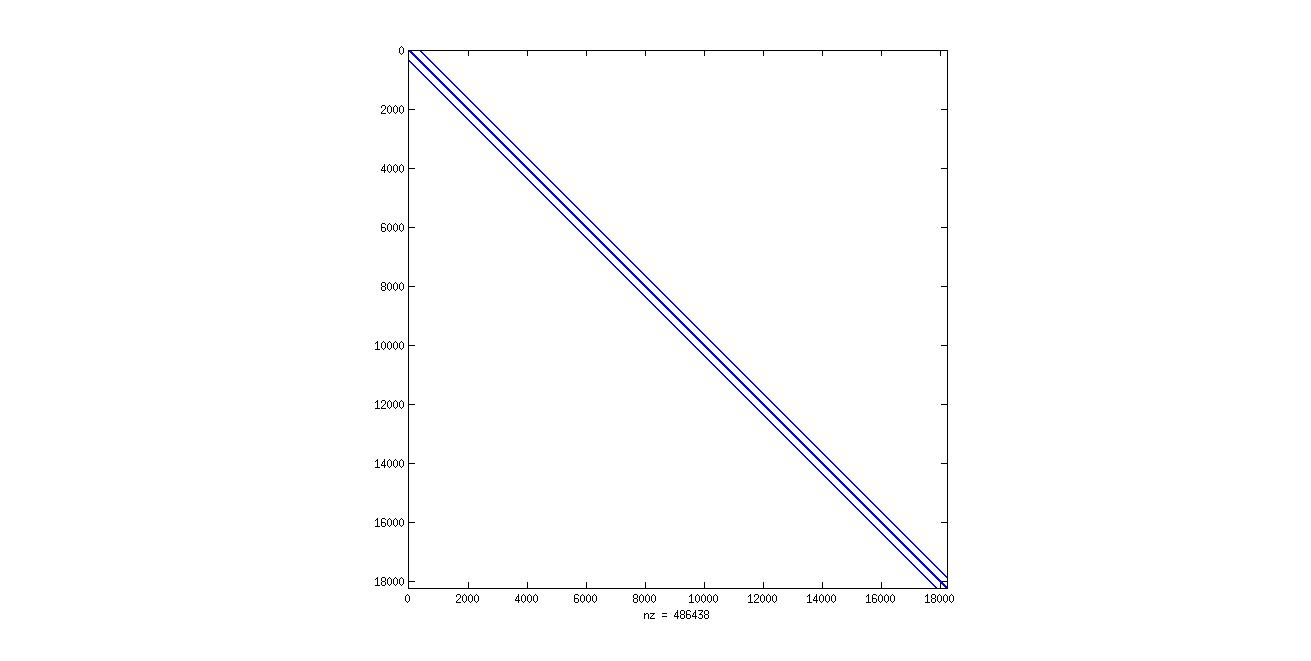
\includegraphics[width=1.8\textwidth]{imago/sparsity.jpg}
\end{figure}
\end{minipage}
\hspace{0.2cm}
\begin{minipage}[t]{0.48\linewidth}
   \begin{figure}[!h]
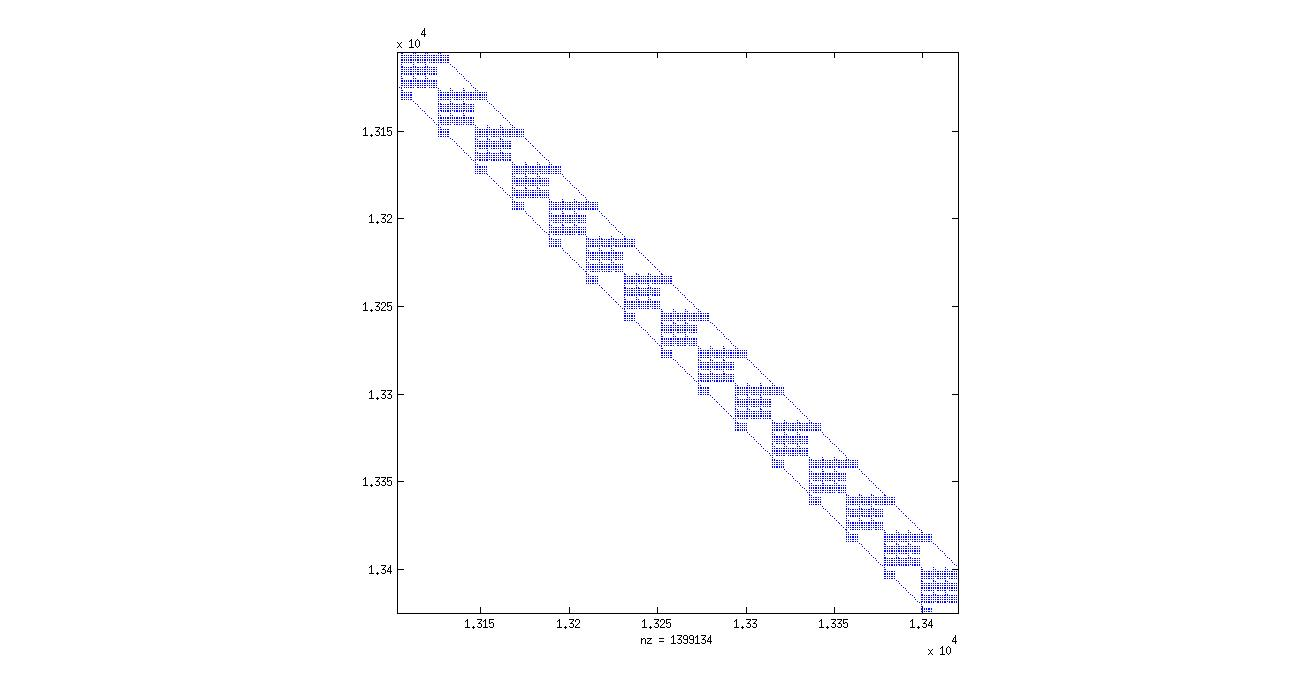
\includegraphics[width=1.8\textwidth]{imago/sparsity2.jpg}
\end{figure}
\end{minipage}
\end{frame}

\begin{frame}
\frametitle{Numerical experiments}
\framesubtitle{Simplified $P_N$ equations}
Properties of matrices:
\begin{itemize}
 \item discretization of $SP_1$ equations
 \item all nonzero diagonal entries
\end{itemize} 
\vspace{0.3cm}
Numerical treatment:
 \begin{itemize}
 \item block Jacobi preconditioning
\end{itemize}

\begin{table}[!h]
\centering
\hspace*{-0.75cm}
\begin{tabular}{|c|c|c|c|c|}
\hline
\textbf{Kind of matrix} & \textbf{size} &
\textbf{nnz}&\textbf{Prec. block size}& \textbf{nnz after prec}\\
\hline
$SP_1$ (a) & 18,207 & 486,438 & 63 & 2,644,523\\ 
\hline
$SP_1$ (b) & 19,941 & 998,631 & 69 & 1,774,786\\
\hline
\end{tabular}
\label{tab:matrices}
\end{table}

\small{[Matrices provided by courtesy by Thomas Evans, Steven Hamilton, Stuart 
Slattery, ORNL]}
\end{frame}

\begin{frame}
\frametitle{Numerical experiments}
\framesubtitle{Simplified $P_N$ equations}
 MCSA parameter setting:
 \begin{itemize}
  \item Adjoint method
  \item residual relative tolerance: $\varepsilon_1=10^{-7}$
  \item almost optimal transition probability
  \item maximal \# steps per history: $10$
  \item statistical error-based adaptive parameter: $\varepsilon_2=0.5$
  \item granularity of the adaptive approach: $n_{histories}=1,000$
  \item simulations run in serial mode
 \end{itemize}
\end{frame}

\begin{frame}
\frametitle{Numerical experiments}
\framesubtitle{Simplified $P_N$ equations}
\vspace*{-0.7cm}
\begin{table}[!h]
\centering
\hspace*{-0.5cm}
\begin{tabular}{|c|c|c|c|c|}
\hline
\textbf{matrix} & $\rho(H)$ &
$\rho(H^*)$&relative err.& \# iterations \\
\hline
$SP_1$ (a) & 0.9779 & 0.9758 & $9.97\cdot 10^{-6}$ & 340 \\ 
\hline
$SP_1$ (b) & 0.9798 & 0.9439 & $3.89\cdot 10^{-5}$ & 209\\
\hline
\end{tabular}
\label{tab:MCSA_SPN}
\end{table}

\vspace*{-0.5cm}
\begin{minipage}[t]{0.48\linewidth}
\begin{figure}[!h]
\hspace*{-1.1cm}
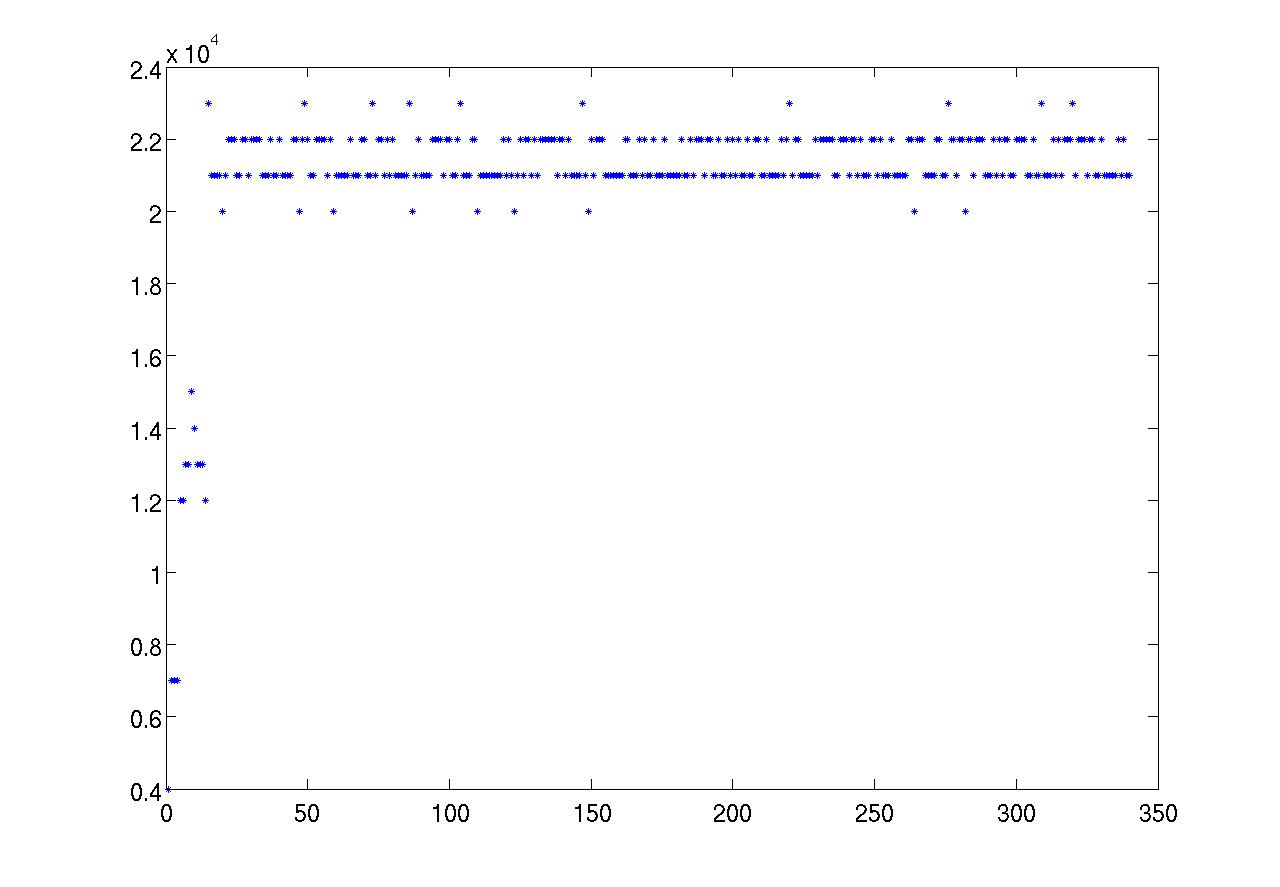
\includegraphics[width=1.1\textwidth]{imago/nwalks1.jpg}
\vspace*{-0.3cm}
\caption{\tiny{\# histories for (a) at each iteration.}}
\label{nwalks1}
\end{figure}
\end{minipage}
\begin{minipage}[t]{0.48\linewidth}
\begin{figure}[!h]
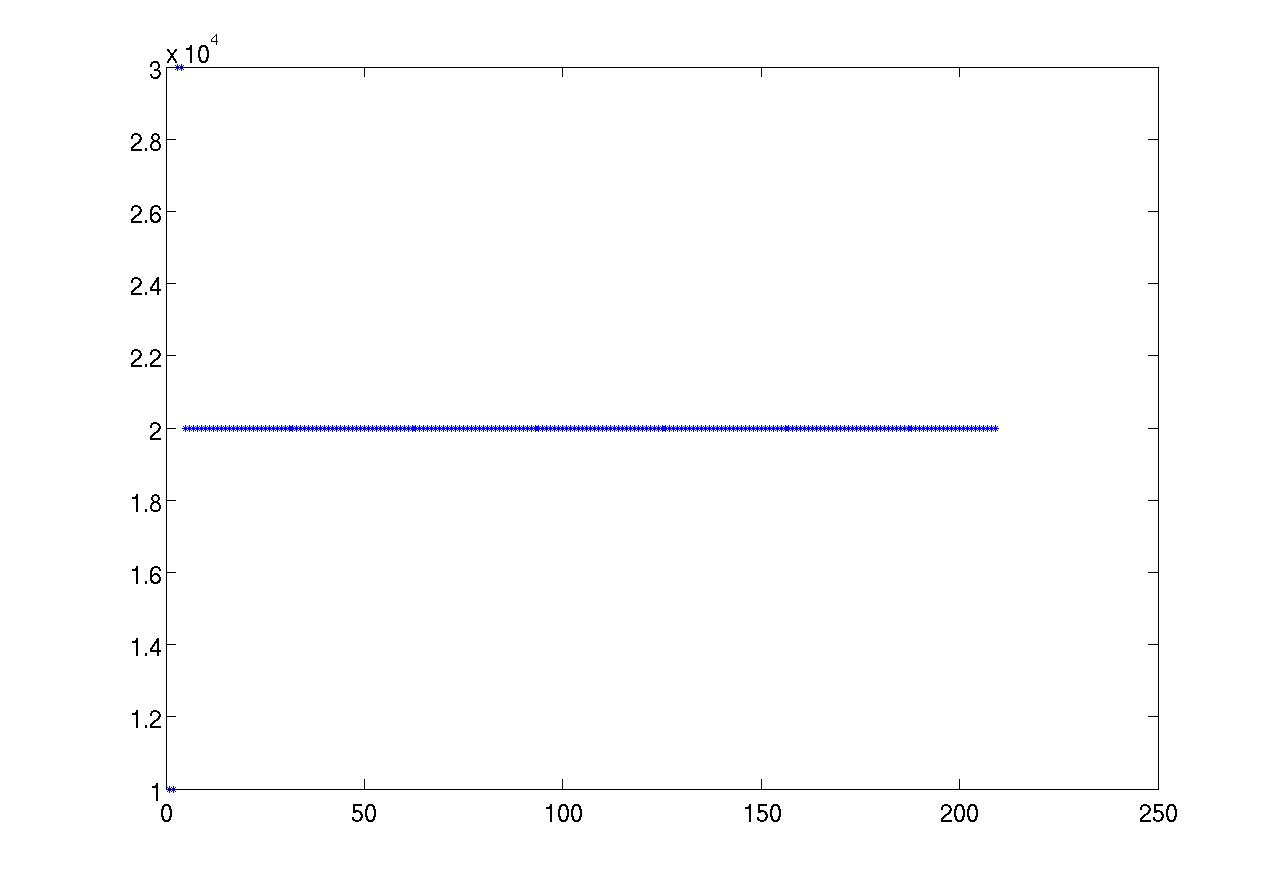
\includegraphics[width=1.1\textwidth]{imago/nwalks2.jpg}
\vspace*{-0.3cm}
\caption{\tiny{\# histories for (b) at each 
iteration.}}
\label{nwalks2}
\end{figure}
\end{minipage}
\end{frame}


\begin{frame}
\frametitle{Numerical experiments}
\framesubtitle{Simplified $P_N$ equations}
Issues raised for a general $SP_N$ matrix:
\begin{itemize}
 \item hard to find a block Jacobi preconditioner s.t. $\rho(H^*)<1$ for every 
$SP_N$ problem
 \item attempt to use Approximate Inverse preconditioners was not effective
 \begin{itemize}
 \item for sparse preconditioners $\rho(H^*)<1$ is not respected
 \end{itemize}
 \item attempt to use ILU preconditioners was not effective
 \begin{itemize}
 \item for ILU(0) we got $\rho(H^*)>1$
 \item massive fill-in with ILUT
 \end{itemize}
 \item reordering and scaling did not facilitate the convergence requirements
\end{itemize}
\end{frame}

\begin{frame}
\frametitle{Numerical experiments}
\framesubtitle{Diagonally dominant matrices}
Set of matrices obtained by a diagonal shift of matrices associated with 
$SP_1$, 
$SP_3$ and $SP_5$ equations.

\[
 (A+sD),\quad s\in \mathbb{R}^+, \quad D=diag(A).
\]

All the matrices have been turned into s.d.d. by columns.

\begin{table}[!h]
\centering
\hspace*{-0.5cm}
\begin{tabular}{|c|c|c|c|c|}
\hline
\textbf{Initial matrix} & $ s $ &
$\rho(H)$ & $Forward - \rho(H^*)$ &$ Adjoint - \rho(H^*)$ \\
\hline
$SP_1$ (a) & 0.3 & 0.7597 & 0.7441 & 0.6983\\ 
\hline
$SP_1$ (b) & 0.4 & 0.7046 & 1.1448 & 0.5680\\
\hline
$SP_3$ & 0.9 & 0.5869 & 0.4426 & 0.3727\\
\hline
$SP_5$ & 1.6 & 0.5477 & 0.3790 & 0.3431\\
\hline
\end{tabular}
\label{tab:shift_spectra}
\end{table}
\end{frame}


\begin{frame}
\frametitle{Numerical experiments}
\framesubtitle{Diagonally dominant matrices}
\[
 (A+sD),\quad s\in \mathbb{R}^+, \quad D=diag(A).
\]

\begin{table}[!h]
\centering
\hspace*{-0.8cm}
\begin{tabular}{|c|c|c|c|c|}
\hline
\textbf{matrix} & nnz & $s$ &relative err.& \# iterations \\
\hline
$SP_1$ (a) & 486,438 & 0.3 & $6.277\cdot 10^{-7}$ & 36 \\ 
\hline
$SP_1$ (b) & 998,631 & 0.4 & $9.885\cdot 10^{-7}$ & 21 \\
\hline
$SP_3$  & 846,549 & 0.9 & $5.919\cdot 10^{-7}$ & 18 \\ 
\hline
$SP_5$  & 1,399,134 & 1.6 & $4.031\cdot 10^{-7}$ & 19 \\
\hline
\end{tabular}
\label{tab:MCSA_diag_shift}
\end{table}

\end{frame}


\begin{frame}
\frametitle{Numerical experiments}
\framesubtitle{Diagonal shift}

Strict diagonally dominance is a sufficient condition for convergence but 
not necessary.
\[
 (A+sD),\quad s\in \mathbb{R}^+, \quad D=diag(A)
\]

such that $\rho(H)<1$ and $\rho(H^*)<1$.
\begin{table}[!h]
\centering
\hspace*{-0.5cm}
\begin{tabular}{|c|c|c|c|c|}
\hline
\textbf{Initial matrix} & $ s $ &
$\rho(H)$ & $Forward - \rho(H^*)$ &$ Adjoint - \rho(H^*)$ \\
\hline
$SP_1$ (a) & 0.2 & 0.8230 & 0.8733 & 0.8195\\ 
\hline
$SP_1$ (b) & 0.2 & 0.8220 & 1.5582 & 0.7731\\
\hline
$SP_3$ & 0.3 & 0.8126 & 0.9459 & 0.7961\\
\hline
$SP_5$ & 0.7 & 0.8376 & 0.8865 & 0.8026\\
\hline
\end{tabular}
\label{tab:nondd_shift_spectra}
\end{table}
\end{frame}

\begin{frame}
\frametitle{Numerical experiments}
\framesubtitle{Diagonal shift}
\[
 (A+sD),\quad s\in \mathbb{R}^+, \quad D=diag(A).
\]
\begin{table}[!h]
\centering
\hspace*{-0.5cm}
\begin{tabular}{|c|c|c|c|}
\hline
\textbf{matrix} & $s$ &relative err.& \# iterations\\
\hline
$SP_1$ (a) & 0.2 & $6.394\cdot 10^{-7}$ & 48 \\ 
\hline
$SP_1$ (b) & 0.2 & $2.59\cdot 10^{-6}$ & 36 \\
\hline
$SP_3$  & 0.3 & $5.35 \cdot 10^{-7}$ & 45 \\ 
\hline
$SP_5$  & 0.7 & $4.21\cdot 10^{-7}$ & 70 \\
\hline
\end{tabular}
\label{tab:MCSA_nodd_diag_shift}
\end{table}
\end{frame}


\end{document}